% Created 2011-04-26 Tue 04:05

\documentclass[english,10pt,presentation]{beamer}
\usepackage[english]{babel}
\usepackage[utf8]{inputenc}
\usepackage[T1]{fontenc}
\mode<article>
{
  \usepackage{times}
  \usepackage{mathptmx}
  \usepackage[left=1.5cm,right=6cm,top=1.5cm,bottom=3cm]{geometry}
}
\usepackage{fancybox}
\usepackage{multimedia}
\usepackage{colortbl}
\usepackage{yfonts}
\usepackage{colortbl}
\usepackage{translator}
\usepackage{times}
\usepackage{fixltx2e}
\usepackage{graphicx}
\usepackage{longtable}
\usepackage{float}
\usepackage{wrapfig}
\usepackage{soul}
\usepackage{textcomp}
\usepackage{marvosym}
\usepackage{wasysym}
\usepackage{latexsym}
\usepackage{amssymb}
\usepackage{amsmath}
\usepackage{amsfonts}
\usepackage{ifthen}
\usepackage{mypgf}
\usepackage{hyperref}

\usepackage{fixltx2e}
\usepackage{graphicx}
\usepackage{longtable}
\usepackage{float}
\usepackage{wrapfig}
\usepackage{soul}
\usepackage{textcomp}
\usepackage{marvosym}
\usepackage{wasysym}
\usepackage{latexsym}
\usepackage{amssymb}
\usepackage{amsmath}
\usepackage{amsfonts}
\usepackage{ifthen}
\usepackage{hyperref}
\usepackage{mypgf}
\usepackage{algorithm2e}
\providecommand{\alert}[1]{\textbf{#1}}

\title{Implementation of Contracting Curve Density Algorithm for Applications in Personal Robotics}
\author{Shulei Zhu}
\date{\today}

\usetheme{dimilar}\usecolortheme{rose}
\begin{document}

\maketitle

\begin{frame}
\frametitle{Outline}
\setcounter{tocdepth}{2}
\tableofcontents
\end{frame}

\section{Motivation}
\label{sec-1}
\begin{frame}
\frametitle{Motivation}
\label{sec-1_1}
\begin{alertblock}{Some challenging task in personal robotics}
\label{sec-1_1_1}
\begin{itemize}

\item Image segmentation\\
\label{sec-1_1_1_1}%
\item Pose estimation\\
\label{sec-1_1_1_2}%
\item Object recognition and tracking\\
\label{sec-1_1_1_3}%
\end{itemize} % ends low level
\end{alertblock}
\begin{itemize}

\item Model-based methods: these problems require much information external to the image\\
\label{sec-1_1_2}%
\item Curve-fitting process: a crucial part of these problems\\
\label{sec-1_1_3}%
\end{itemize} % ends low level
\begin{exampleblock}{Requirements}
\label{sec-1_1_4}
\begin{itemize}

\item Robustness: stable in texture, clutter, poor contrast environment\\
\label{sec-1_1_4_1}%
\item Accuracy: high sub-pixel accuracy\\
\label{sec-1_1_4_2}%
\item Efficiency: time-constrained, limited computer hardware resources in personal robotics\\
\label{sec-1_1_4_3}%
\end{itemize} % ends low level
\end{exampleblock}
\end{frame}
\section{Outline of the talk}
\label{sec-2}
\begin{frame}
\frametitle{Outline of the talk}
\label{sec-2_1}
\end{frame}
\section{How the original CCD works?}
\label{sec-3}
\begin{frame}
\frametitle{How the original CCD works?}
\label{sec-3_1}

   \begin{figure}[htb]
   \centering
   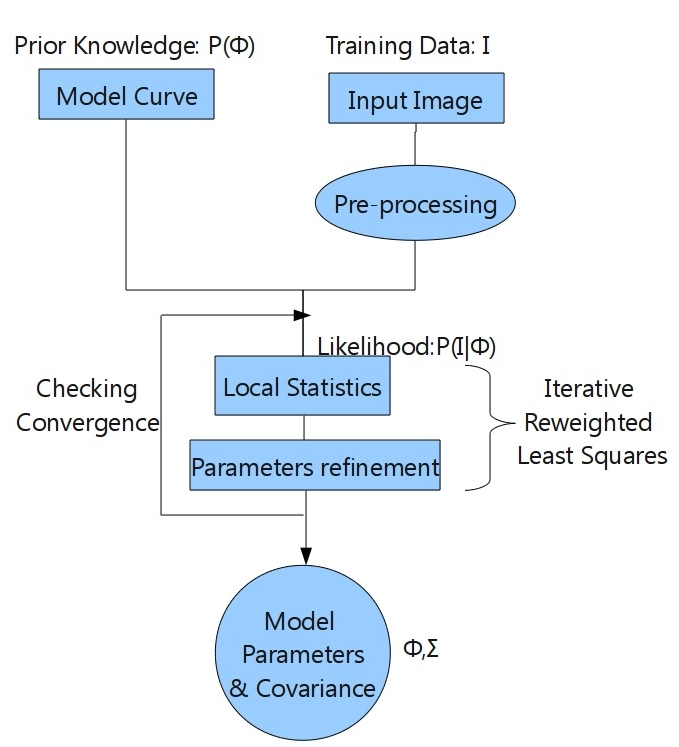
\includegraphics[width=6cm,angle=0]{./flowchart.jpg}
   \caption{\label{fig: flowchart}the CCD algorithm}
   \end{figure}
\end{frame}
\begin{frame}
\frametitle{Sketch of the CCD algorithm}
\label{sec-3_2}
\begin{exampleblock}{Basic steps of the CCD algorithm}
\label{sec-3_2_1}
\begin{itemize}

\item Contour initialization\\
\label{sec-3_2_1_1}%
\item Learning of local statistics\\
\label{sec-3_2_1_2}%
\item Refinement of model parameters\\
\label{sec-3_2_1_3}%
\begin{figure}[htb]
     \centering
     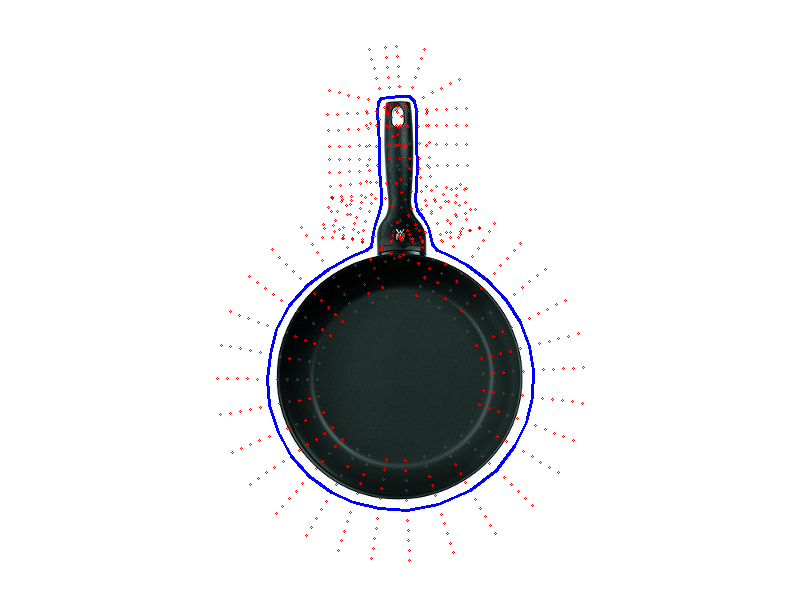
\includegraphics[width=6cm,angle=0]{./pan_contour.jpg}
     \caption{\label{fig:contour}The contour of a pan}
     \end{figure}
\end{itemize} % ends low level
\end{exampleblock}
\end{frame}
\begin{frame}
\frametitle{An alternative view of the CCD algorithm}
\label{sec-3_3}
\begin{exampleblock}{Bayesian logistic regression}
\label{sec-3_3_1}
\begin{itemize}

\item Evaluation of conditional distribution $p(\Phi|\mathbf{I})$
\label{sec-3_3_1_1}%
\begin{displaymath}
p(\Phi|\mathbf{I})
\propto \underbrace{p(\mathbf{I}|\mathbf{m}_{\Phi},
\Sigma_{\Phi})}_{\mathrm{local\ statistics}}\quad\times\quad
\underbrace{p(\Phi)}_{\mathrm{prior\ distribution}}
\end{displaymath}

\item Goal: MAP (maximum a posteriori probability) solution of cost function $\mathcal{Q}(\Phi)$
\label{sec-3_3_1_2}%
\begin{displaymath}
\mathcal{Q}(\Phi) = \underset{\Phi}{\arg\max}\ \mathrm{ln}(p(\Phi|\mathbf{I}))
\end{displaymath}
Approach: iterative reweighted least  squares (IRLS) e.g. Gaussian
Newton method, SVM
\end{itemize} % ends low level
\end{exampleblock}
\end{frame}
\begin{frame}
\frametitle{An alternative view of the CCD algorithm}
\label{sec-3_4}
\begin{exampleblock}{A classification problem}
\label{sec-3_4_1}

    \begin{figure}[htb]
    \centering
    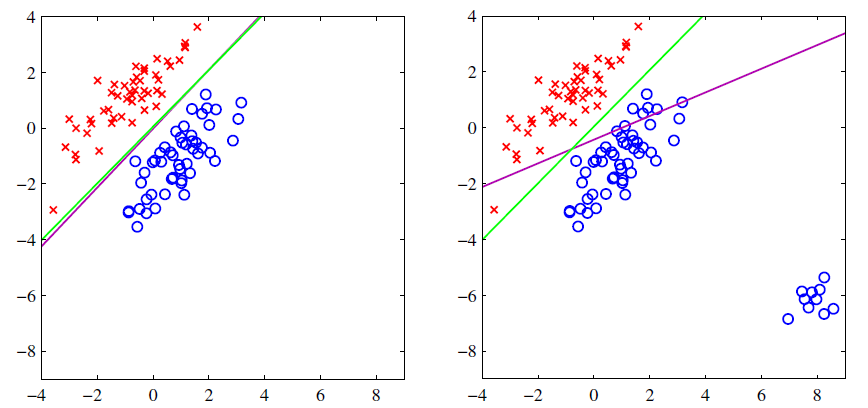
\includegraphics[width=9cm,angle=0]{./images/classification.png}
    \caption{\label{fig:class}A classification problem}
    \end{figure}
\end{exampleblock}
\end{frame}
\section{Related work}
\label{sec-4}
\begin{frame}
\frametitle{3-4 papers}
\label{sec-4_1}
\end{frame}
\section{Improvements of the original algorithm}
\label{sec-5}
\begin{frame}
\frametitle{Quadratic and Cubic B-spline curves}
\label{sec-5_1}
\begin{exampleblock}{B-spline curves}
\label{sec-5_1_1}

\begin{equation*}
  \mathbf{C}(u) =  \sum_{i=0}^{m-n-2} P_{i} B_{i,n}(u) \mbox{ , } u \in [u_{n},u_{m-n-1}]
\end{equation*}
\begin{figure}[htb]
\centering
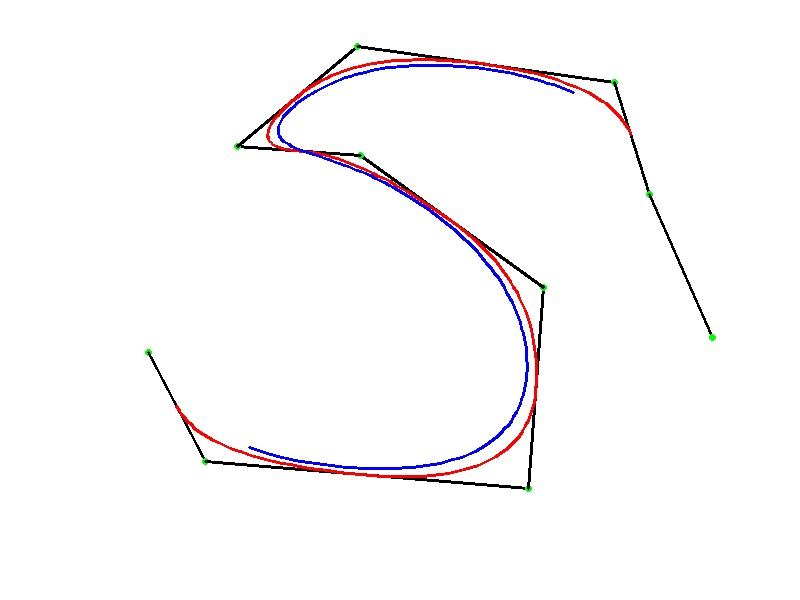
\includegraphics[width=6cm,angle=0]{./bspline.jpg}
\caption{\label{fig: bspline}B-spline curves of degree = 1, 2, 3}
\end{figure}
\end{exampleblock}
\end{frame}
\begin{frame}
\frametitle{Logitic and Probit function}
\label{sec-5_2}
\begin{columns}
\begin{column}{0.5\textwidth}
\begin{exampleblock}<1->{Logistic function}
\label{sec-5_2_1}

    \begin{figure}[htb]
    \centering
    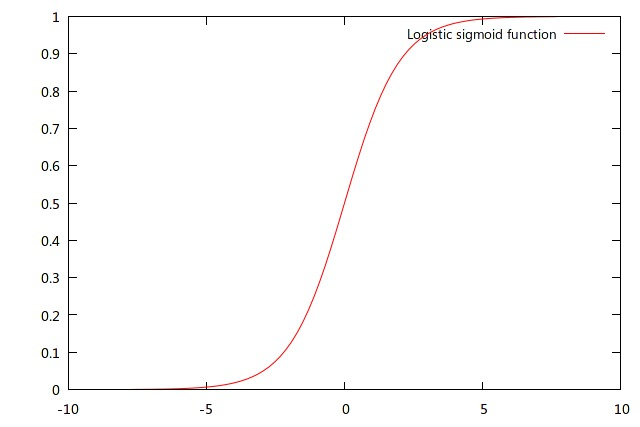
\includegraphics[width=4cm,angle=0]{./logistic.jpg}
    \caption{\label{fig:log}Logistic function}
    \end{figure}
\begin{displaymath}
f(\cdot) = \frac{1}{1+\mathrm{e}^{-x}}
\end{displaymath}
\end{exampleblock}
\end{column}
\begin{column}{0.5\textwidth}
\begin{exampleblock}<2->{Probit function}
\label{sec-5_2_2}

    \begin{figure}[htb]
    \centering
    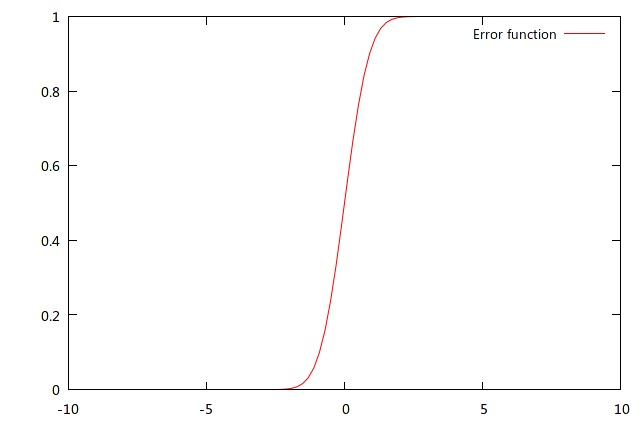
\includegraphics[width=4cm,angle=0]{./erf.jpg}
    \caption{\label{fig: probit}Probit function}
    \end{figure}
\begin{displaymath}
f(\cdot) = \frac{1}{2}(\frac{1}{\sqrt{2}}erf(x) + 1)
\end{displaymath}
\end{exampleblock}
\end{column}
\end{columns}
\end{frame}
\begin{frame}
\frametitle{Three-dimensional Affine Shape-space}
\label{sec-5_3}
\begin{columns}
\begin{column}{0.5\textwidth}
\begin{block}{Parallax effect in two-dimensional affine shape-space}
\label{sec-5_3_1}

    \begin{figure}[htb]
    \centering
    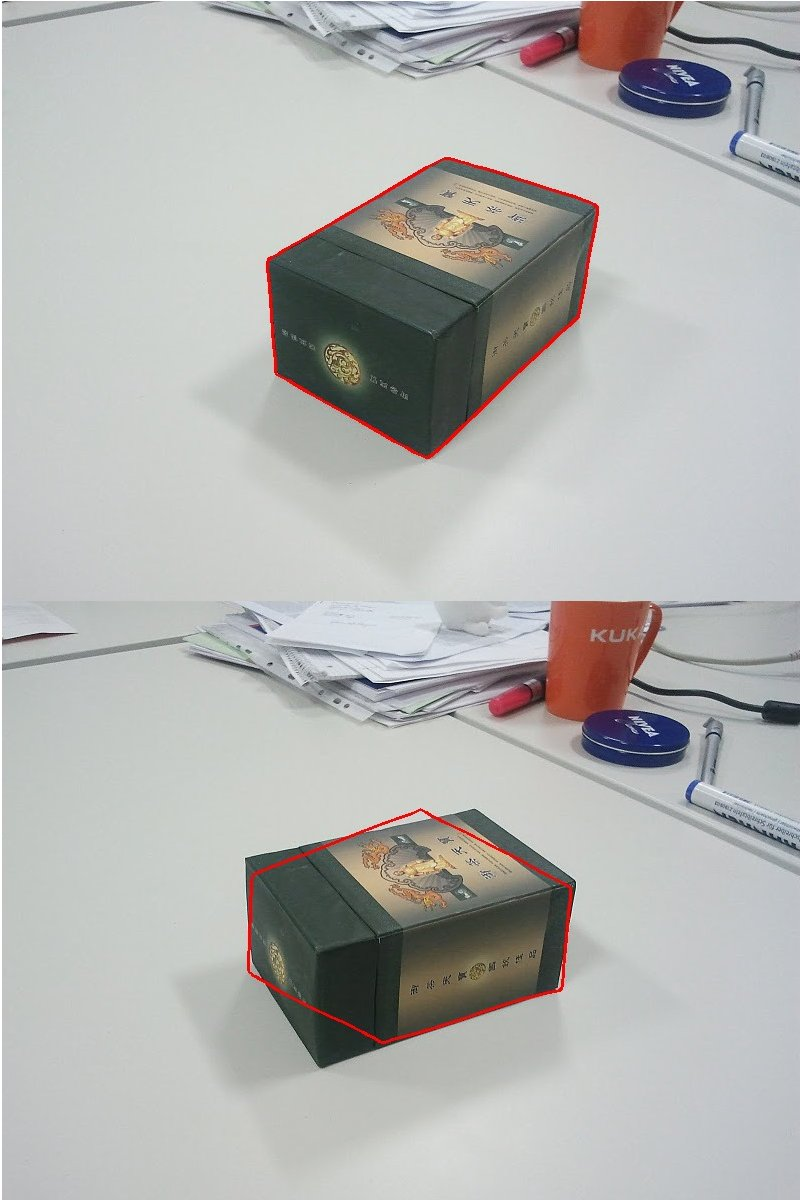
\includegraphics[width=3cm,angle=0]{./planar.jpg}
    \caption{\label{fig:parallax effect}Parallax effect}
    \end{figure}
\end{block}
\end{column}
\begin{column}{0.5\textwidth}
\begin{block}{Three-dimensional affine shape-space}
\label{sec-5_3_2}

    \begin{figure}[htb]
    \centering
    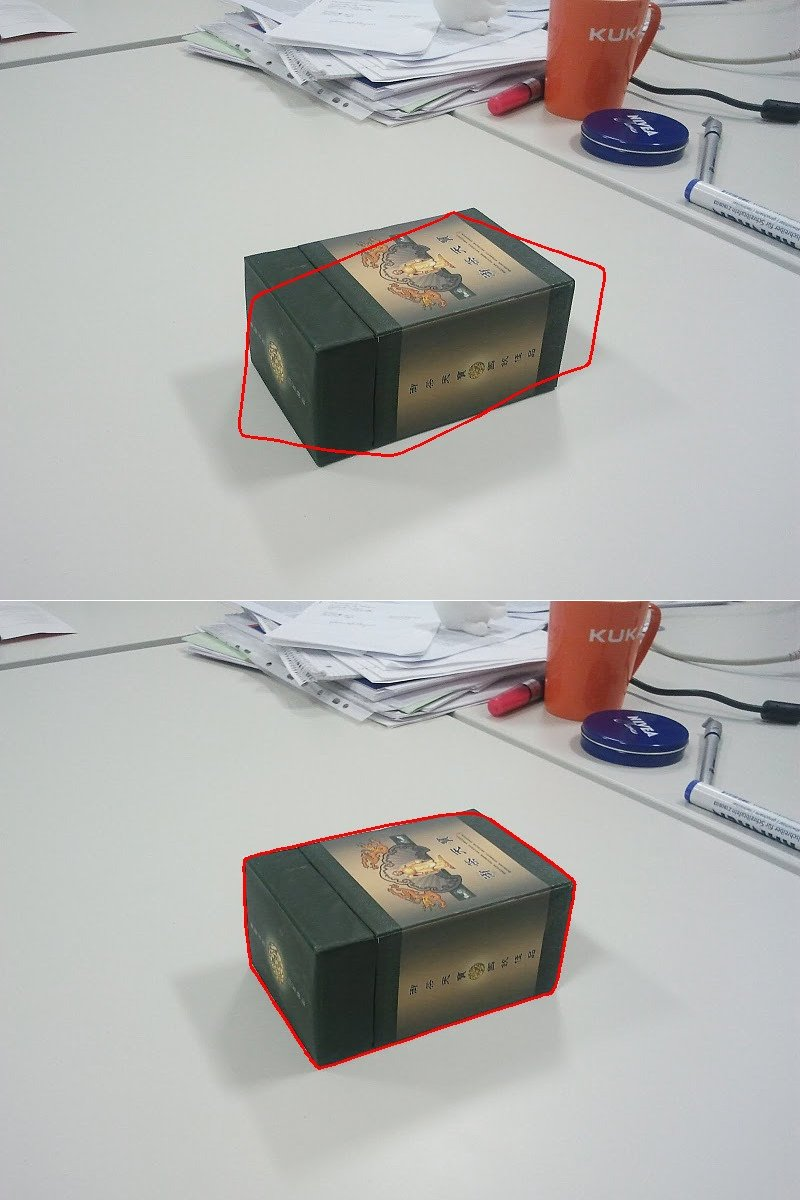
\includegraphics[width=3cm,angle=0]{./nonplanar.jpg}
    \caption{\label{fig:3das}Three-dimensional affine shape-space}
    \end{figure}
\end{block}
\end{column}
\end{columns}
\end{frame}
\begin{frame}
\frametitle{Initialization from SIFT Features}
\label{sec-5_4}
\begin{block}{Initialization from SIFT Features}
\label{sec-5_4_1}

    \begin{figure}[htb]
    \centering
    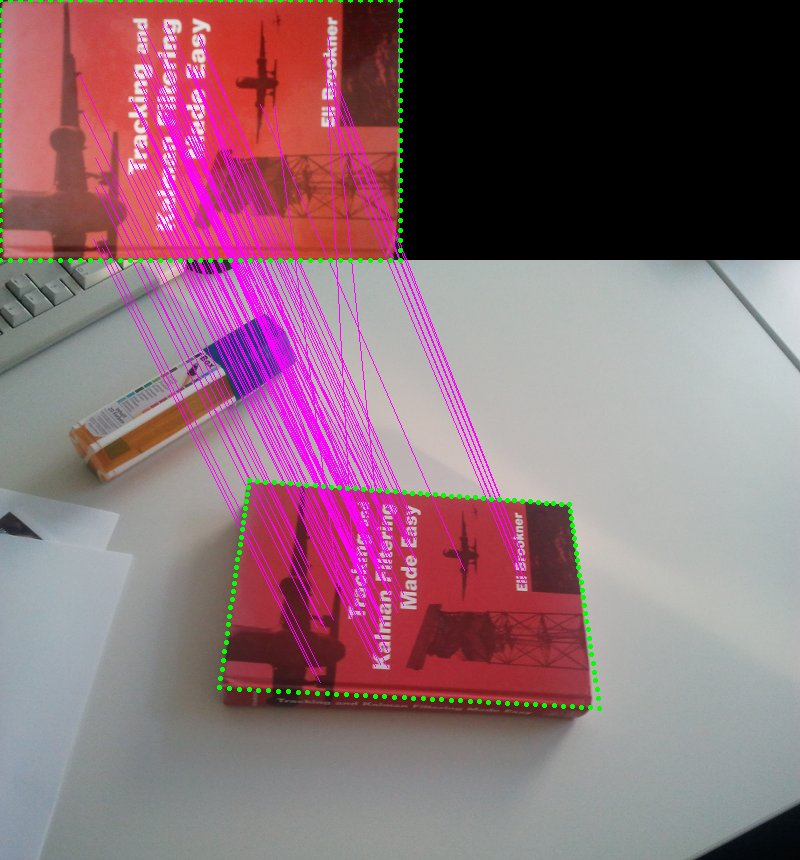
\includegraphics[width=6cm,angle=0]{./sift.jpg}
    \caption{\label{fig:sift}Initialization from SIFT Features}
    \end{figure}
\end{block}
\end{frame}
\section{The CCD tracker}
\label{sec-6}
\begin{frame}
\frametitle{algorithm}
\label{sec-6_1}
\end{frame}
\section{Results of the experiments}
\label{sec-7}
\begin{frame}
\frametitle{manually initialization}
\label{sec-7_1}
\end{frame}
\begin{frame}
\frametitle{initialization from SIFT}
\label{sec-7_2}
\end{frame}
\section{Summary and Future work}
\label{sec-8}
\section{Thanks}
\label{sec-9}

\end{document}
